\documentclass[electronic,oldfontcommands]{kthesis}

%%%%%%%%%%%%%%%%%
%%%% PACKAGES %%%
%%%%%%%%%%%%%%%%%
\usepackage[utf8]{inputenc}
\usepackage[swedish,english]{babel}
\usepackage{csquotes}
\usepackage[inline]{enumitem}
\usepackage{caption}   % to align the table caption to the right/left

% headers
\usepackage{fancyhdr}
\pagestyle{fancy}
\fancyhf{}
\fancyhead[LE,RO]{\thepage}
\fancyhead[RE]{\leftmark}
\fancyhead[LO]{\rightmark}

\usepackage{lscape}
\usepackage{hyperref}  %for references
\usepackage{amsmath,mathrsfs}
\usepackage{amssymb}  % assumes amsmath package installed
\usepackage{epstopdf}
\usepackage{subfig}
\usepackage{epigraph}
% \usepackage{cite}
\usepackage[
  giveninits=false,
  style=ieee,
  sorting=none,
  sortcites,
  hyperref,
  mincitenames=1,
  maxcitenames=2,
  maxbibnames=10,
  minbibnames=1,
  citestyle=numeric-comp, % for [1, 2] instead of [1], [2]
  backend=biber
]{biblatex}
\bibliography{Refs.bib,bibliography/bibliography.bib}

% included papers
\DeclareBibliographyCategory{thesispapers}
\addtocategory{thesispapers}{Olguin:DemoScaling2018}
\addtocategory{thesispapers}{Olguin:EdgeDroid2019}
\addtocategory{thesispapers}{Olguin:ImpactWCA2021}
\addtocategory{thesispapers}{CLEAVE2022}

\usepackage{cleveref}
\usepackage{graphicx}
\usepackage{bm}	%Command \bm{make bold}
\usepackage{algorithm}
\usepackage{algpseudocode}
\usepackage{algpascal}
\usepackage{multicol}
\usepackage[x11names]{xcolor}
\usepackage{lipsum}
\usepackage[printonlyused]{acronym}
\usepackage{booktabs}
\usepackage{graphicx}
\usepackage[binary-units]{siunitx}
\DeclareSIUnit{\belmilliwatt}{Bm}
\DeclareSIUnit{\dBm}{\deci\belmilliwatt}

\usepackage{xcolor}
\usepackage{pagecolor}
\usepackage{tikz}
\usetikzlibrary{tikzmark,calc,decorations.pathreplacing,shapes,arrows.meta,positioning,automata}
\usepackage[export]{adjustbox}
\usepackage{pgf-umlsd}
\input{publications/2018DemoScalingOnTheEdge/pgf-umlsd-ex.tex}

\newcommand{\Depth}{2}
\newcommand{\Height}{2}
\newcommand{\Width}{2}

\renewcommand{\labelitemi}{\textcolor{IndianRed3}{\bfseries\textbullet}}

% fancy chapters
\usepackage[Sonny]{fncychap}
\ChNameVar{\normalfont\large\rmfamily}
\ChNumVar{\normalfont\rmfamily\bfseries}
\ChTitleVar{\normalfont\rmfamily\huge}

\usepackage{xparse}
\NewDocumentCommand{\thesischapter}{o m m}{%
   \IfNoValueTF{#1}
     {\chapter[#2]{#2\origtitle{#3}}}
     {\chapter[#1]{#2\origtitle{#3}}}%
}
\newcommand\origtitle[1]{\\
  \parbox{\textwidth}{\normalsize\vspace*{2\baselineskip}#1}}


\usepackage{appendix}
\usepackage{hyperref}

\newenvironment{dedication}{\cleardoublepage\null\vspace{\stretch{1}}\begin{flushright}\itshape}{\end{flushright}\vspace{\stretch{2}}\null}

\newcommand{\citeallnames}
{\AtNextCite{\defcounter{maxnames}{99}}\citename}

\makeatletter
\newcommand{\int@suppauthtitle}{%
  \def\ifciteibid{\@secondoftwo}%
  \renewbibmacro*{cite:name}{}%
  \renewbibmacro*{cite:idem}{}%
  \renewbibmacro*{author}{}%
  \renewbibmacro*{editor+others}{}%
  \renewbibmacro*{translator+others}{}%
  \renewbibmacro*{url}{}%
  \renewbibmacro*{in:}{Refereed article published in\\}%
  \renewbibmacro*{title}{}%
  \renewbibmacro*{annotation}{}%
  \renewbibmacro*{journal}{%
    \ifboolexpr{
      test {\iffieldundef{journaltitle}}
      and
      test {\iffieldundef{journalsubtitle}}
    }
    {}
    {\printtext[journaltitle]{%
       \normalfont{Refereed article published in}\\
       \printfield[titlecase]{journaltitle}%
       \setunit{\subtitlepunct}%
       \printfield[titlecase]{journalsubtitle}}}}
  }%

\newcommand{\suppauthtitle}{\AtNextCite{\int@suppauthtitle}}
\makeatother

\definecolor{titlecolor}{HTML}{ECCEF5}

\newcommand{\thesispaper}[2]
{%
\begin{titlingpage*}
\newpagecolor{titlecolor}
\chapter[#1]{\citefield{#2}{title}}

\begin{flushright}
{\citeallnames{#2}{author}}

\vspace{3em}

\suppauthtitle\fullcite{#2}
\end{flushright}

\thispagestyle{empty}
\clearpage%
\hspace{0pt}\vfill%
\noindent\textcopyright~{\citeyear{#2}~\citelist{#2}{publisher}}

\noindent{Layout has been revised for thesis consistency.}

\vfill\hspace{0pt}%
\end{titlingpage*}%
\restorepagecolor%
}


%%%%%%%%%%%%%%%%%%%%%%%%%%%%%%%%%%%%%%%
%%%%%%%%% Document starts here %%%%%%%%
%%%%%%%%%%%%%%%%%%%%%%%%%%%%%%%%%%%%%%%
\begin{document}

%%%%%%%%%%%%%%%%%%%%%%%%%%%%%%%%%%%%%%%%%%
%%%%%% First and second pages %%%%%%%%%%%%
%%%%%%%%%%%%%%%%%%%%%%%%%%%%%%%%%%%%%%%%%%
\title{ Thesis Title }
\subtitle{\textbf{sub-title}}
\author{Manuel {Osvaldo Jesús} {Olguín Muñoz}}
\date{\today}
\thesistype{Doctoral Thesis}
\imprint{Stockholm, Sweden, \the\year{}}
\examen{Teknologie doktorexamen i elektroteknik}
\disputationsdatum{fredagen den 18 januari 2020 klockan 14.00}
\disputationslokal{Sal F3, Lindstedtsvägen 26, Kungliga Tekniska Högskolan, Stockholm}
\publisher{Universitetsservice US AB}
\address{%
	KTH Royal Institute of Technology\\%
	School of Electrical Engineering and Computer Science\\%
	Division of Information Science and Engineering\\%
	SE-10044 Stockholm\\%
	Sweden%
}
\isbn{ISBN 100-}
%\issn{ISSN XXX} % No longer used at KTH
\trita{TRITA-EECS-AVL-2020:4}
\kthlogo{KTHLogo}

% Create title page using info above
\maketitle

\frontmatter % Pages i, ii, iii, iv, v etc.

\phantomsection\addcontentsline{toc}{chapter}{Abstract}
\begin{abstract}
    Cloud Computing, with its globally-accessible nature and virtually unlimited scalability, has revolutionized our daily lives since its widespread adoption in the early 2000s.
    It allows us to access our documents anywhere, keep in contact with our friends, back up our photos, and even remote-control some of our appliances.
    Despite this, Cloud Computing has limitations when it comes to novel applications requiring real-time processing or low-latencies.
    Applications such as \glspl{CPS} or mobile \gls{XR}, which in turn also have great transformative potential, are unable to run on the Cloud.

    Edge Computing is emerging as a potential solution to these limitations by bringing computation and data processing closer to the edge of the network, thereby reducing latency and enabling real-time decision making.
    The combination of Edge Computing and modern mobile network technologies such as 5G offers potential for massive deployments of latency-sensitive applications.
    However, scaling and understanding these deployments poses important challenges such the optimization of latency through multiple processing steps and trade-offs in wireless system choice, protocols, hardware, and algorithms.
    Existing approaches have so far been unsuccessful in capturing the complex effects arising from the interplay between network and compute in these systems.

    This dissertation addresses the challenge of performance evaluation of Edge Computing and the applications enabled by this paradigm with two key contributions to literature.
    First, a methodological approach to experimentally studying the trade-offs between system responsiveness and resource consumption in Edge-bound latency-sensitive applications such as \glspl{CPS} and \gls{XR} is introduced.
    These applications and systems feature characteristics, such as tight interaction with the physical world and the involvement of humans, that make them challenging to study through simulated approaches or analytical modeling.
    The approach presented in this thesis involves therefore the emulation of the client-side workload while maintaining the real server-side process and network stack to retain the realism of network and compute effects.

    Next, an exploration of the requirements for realism in the emulation is presented.
    Further, this work discusses the extent to which realism in the emulation can open new avenues for optimization of these systems.
    To this end, the first-ever realistic model of human timings for a particular class of \gls{MAR} applications is provided. 
    The model is combined with a mathematical framework to study the potential for optimization in these applications.

    Results indicate that the methodology introduced in this work offers advantages over existing methods by improving efficiency, repeatability, and replicability.
    By fully integrating workload components into the emulated software domain, this methodology reduces complexity while still capturing complex effects of network and compute factors that are challenging to model.
    This approach represents thus an important contribution to literature, as it consists of a comprehensive method for the performance evaluation of Edge environments, encompassing both the application and the infrastructure.
    Furthermore, results from the exploration into the implications of realism in the emulation suggest that incorporating enhanced realism in client-side emulation can enable the implementation of optimization approaches that would otherwise be infeasible.
    In particular, this work highlights the significance of considering human behavior and reactions in addition to system-related metrics and performance optimizations in the context of \gls{MAR}.
\end{abstract}

\vspace{3em}

\setlength{\leftskip}{0.3 cm} \textbf {Keywords:} Lorem, Ipsum, Dolor, Sit, Amet
\todo[inline]{Keywords!}

%%%%%%%%%%%%%%%%%%%%%%%%%%%%%%%%%%%%%%%%
%%%%%%%% SWEDISH ABSTRACT %%%%%%%%%%%%%%
%%%%%%%%%%%%%%%%%%%%%%%%%%%%%%%%%%%%%%%%
\newpage
\selectlanguage{swedish}
\phantomsection\addcontentsline{toc}{section}{Abstract (Swedish)}
\glsresetall%
\begin{abstract}
    Cloud Computing, med sin globalt tillgängliga natur och praktiskt taget obegränsade skalbarhet, har revolutionerat våra dagliga liv sedan dess allmänna antagande i början av 2000-talet.
    Det gör det möjligt för oss att få tillgång till våra dokument var som helst, hålla kontakt med våra vänner, säkerhetskopiera foton, och till och med fjärrstyra våra hushållsapparater. 
    Trots detta har Cloud Computing begränsningar när det gäller nya applikationer som kräver realtidsbehandling eller låg latens.
    Applikationer som cyberfysiska system (engelska \emph{\gls{CPS}}) eller mobilt utvidgad verklighet (engelska \emph{\gls{XR}}), som i sin tur också har stor omvandlingspotential, kan inte köras på molnet.

     Edge Computing är en potentiell lösning på dessa begränsningar som, genom att föra beräkningar och databehandling närmare kanten av nätverket, minskar latensen och möjliggör beslutsfattande i realtid.
     Kombinationen av Edge Computing och moderna mobila nätverksteknologier som 5G erbjuder potential för massiva utrullningar av latenskänsliga applikationer. 
     Men att skala och förstå dessa utrullningar utgör viktiga utmaningar såsom optimering av latens genom flera bearbetningssteg och avvägningar i val av trådlösa system, protokoll, hårdvara och algoritmer.
     Befintliga metoder har hittills inte lyckats fånga de komplexa effekter som uppstår från samspelet mellan nätverk och datorer i dessa system.
     
     Den här avhandlingen tar upp utmaningen med prestationsutvärdering av Edge Computing och applikationerna som möjliggörs av detta paradigm med två viktiga bidrag till litteraturen.
     Först introduceras ett metodologiskt tillvägagångssätt för att experimentellt studera kompromisserna mellan systemrespons och resursförbrukning i latenskänsliga applikationer såsom \glspl{CPS} och \gls{XR} som körs på Edge Computing.
     Dessa applikationer och system har egenskaper, såsom tät interaktion med den fysiska världen och inblandning av människor, som gör dem utmanande att studera genom simulerade tillvägagångssätt eller analytisk modellering.
     Den metod som presenteras i denna avhandling innebär därför emulering av klientsidans arbetsbelastning samtidigt som den verkliga serversidans process och nätverksstacken bibehålls för att bibehålla realismen i nätverks- och datoreffekter.

     Därefter presenteras en utforskning av kraven på realism i emuleringen.
     Vidare diskuterar detta arbete i vilken utsträckning realism i emuleringen kan öppna nya vägar för optimering av dessa system.
     För detta ändamål tillhandahålls den första realistiska modellen av mänskliga tidsbeteenden för en särkild klass av mobilt förstärkt verklighets-applikationer (engelska \emph{\gls{MAR}}).
     Modellen kombineras med ett matematiskt ramverk för att studera potentialen för optimering i dessa applikationer.

     Resultaten indikerar att den metod som introducerats i detta arbete erbjuder fördelar jämfört med befintliga metoder genom att förbättra effektiviteten, repeterbarheten och replikerbarheten.
     Genom att helt integrera arbetsbelastningskomponenter i den emulerade mjukvarudomänen, minskar denna metodik komplexiteten samtidigt som den fångar komplexa effekter av nätverks- och beräkningsfaktorer som är utmanande att modellera.
     Detta tillvägagångssätt representerar således ett viktigt bidrag till litteraturen, eftersom det består av en omfattande metod för prestandautvärdering av Edge Computing-miljöer, som omfattar både applikationen och infrastrukturen.
     Dessutom tyder resultat från utforskningen av implikationerna av realism i emuleringen att inkorporering av förbättrad realism i klientsideemulering kan möjliggöra implementering av optimeringsmetoder som annars skulle vara omöjliga.
     Särskilt framhåller detta arbete betydelsen av att överväga mänskligt beteende och reaktioner utöver systemrelaterade mätvärden och prestandaoptimeringar i samband med \gls{MAR}.

\end{abstract}
\selectlanguage{english}
\glsresetall%
%%%%%%%%%%%%%%%%%%%%%%%%%%%%%%%%%%%%%%%
%%%%%%% List of papers %%%%%%%%%%%%%%%%
%%%%%%%%%%%%%%%%%%%%%%%%%%%%%%%%%%%%%%%
% \chapter{List of Papers}

\nocite{Olguin:DemoScaling2018}
\nocite{Olguin:EdgeDroid2019}
\nocite{Olguin:ImpactWCA2021}
\nocite{CLEAVE2022}
\nocite{Ainur2022}
% \cite{Olguin:ImpactWCA2021}
% \begin{refcontext}[sorting=none]
\printbibliography[
	% env=thesispapers,
	heading=bibintoc,
	title={List of Papers},
	category=thesispapers
]
% \end{refcontext}




% \begin{enumerate}[label=\Roman*]
% 	\item \fullciteall{Olguin:DemoScaling2018}
% 	\item \fullciteall{Olguin:EdgeDroid2019}
% 	\item \fullciteall{Olguin:ImpactWCA2021}
% 	\item \fullciteall{CLEAVE2022}
% \end{enumerate}
%%%%%%%%%%%%%%%%%%%%%%%%%%%%%%%%%%%%%%%
%%%%%%%% ACKNOWLEDGMENT %%%%%%%%%%%%%%%
%%%%%%%%%%%%%%%%%%%%%%%%%%%%%%%%%%%%%%%
\chapter{Acknowledgements}
\noindent \lipsum[1]

\todo[inline]{Acknowledge ChatGPT}

\begin{acronym}
    \acro{CPS}{Cyber-Physical System}
    \acro{NCS}{Networked Control System}
    \acroindefinite{NCS}{an}{a}
    \acro{LAN}{Local-Area Network}
    \acro{WLAN}{Wireless Local-Area Network}
    \acro{KPI}{Key Performance Indicator}
    \acro{WPAN}{Wireless Personal Area Network}
    \acro{CSMA/CD}{Carrier-Sense Multiple Access with Collision Detection}
    \acro{CLEAVE}{ControL bEnchmArking serVice on the Edge}
    \acro{OS}{Operating System}
    \acro{UDP}{User Datagram Protocol}
    \acro{TCP}{Transmission Control Protocol}
    \acro{RMS}{Root Mean Square}
    \acro{RTT}{Round-Trip Time}
    \acro{CI}{Confidence Interval}
    \acro{AP}{Access Point}
    \acro{API}{Application Programming Interface}
    \acro{SSF}{Swedish Foundation for Strategic Research}
    \acro{TECoSA}{Trustworthy Edge Computing Systems and Applications}
    \acro{ABC}{Abstract Base Class}
    \acroplural{ABC}[ABCs]{Abstract Base Classes}
    \acro{URL}{Uniform Record Locator}
    \acro{AWS}{Amazon Web Services}
    \acro{EC2}{Elastic Compute 2}
    \acro{AMI}{Amazon Machine Image}
    \acro{SSH}{Secure Shell}
    \acro{IP}{Internet Protocol}
    \acro{VPN}{Virtual Private Network}
    \acro{NAT}{Network Address Translation}
    \acro{NTP}{Network Time Protocol}
    \acroindefinite{NTP}{an}{a}
    \acro{SDR}{Software-Defined Radio}
    \acroindefinite{SDR}{an}{a}
    \acro{VLAN}{Virtual Local-Area Network}
    \acro{APT}{Advaced Packaging Tool}
    \acro{LTE}{Long-Term Evolution}
    \acro{SSID}{Service Set Identifier}
    \acro{EPC}{Evolved Packet Core}
    \acro{UE}{User Equipment}
    \acro{eNodeB}{Evolved Node B}
    \acro{DNS}{Domain Name System}
    \acro{MNIST}{Modified National Institute of Standards and Technology}
    \acro{HTTP}{Hyper-Text Transfer Protocol}
    \acroindefinite{HTTP}{an}{a}
    \acro{YAML}{YAML Ain't Markup Language}
    \acro{O-RAN}{Open Radio Access Network}
    \acro{FOSS}{Free and Open Source Software}
    \acro{COSMOS}{Cloud enhanced Open Software defined MObile wireless testbed for city-Scale deployment}
    \acro{OMF}{ORBIT Management Framework}
    \acro{POWDER}{Platform for Open Wireless Data-driven Experimental Research}
    \acro{COTS}{Commercial Off-The-Shelves}
    \acro{RF}{Radio-Frequency}
    \acro{VM}{Virtual Machine}
    \acro{REST}{REpresentational Sate Transfer}
    \acro{OS}{Operating System}
    \acro{MaaS}{Metal-as-a-Service}
    \acro{OEDL}{\ac{OMF} Experiment Description Language}
    \acro{RSpec}{Resource Specification}
    \acro{LXC}{LinuX Containers}
    \acro{MEC}{Mobile Edge Computing}
    \acro{USRP}{Universal Software Radio Peripheral}
    \acro{OAI}{OpenAirInterface}
    \acro{NR}{New Radio}
    \acro{FPGA}{Field-Programmable Gate Array}
    \acro{WCA}{Wearable Cognitive Assistance}
    \acro{TTF}{Time-to-Feedback}
    \acro{AR}{Augmented Reality}
    \acro{GPS}{Global Positioning System}
    \acro{QoE}{Quality of Experience}
    \acro{QoS}{Quality of Service}
    \acro{TTF}{Time-to-Feedback}
    \acro{PCA}{Principal Component Analysis}
\end{acronym}

\mainmatter % Pages 1, 2, 3...

\tableofcontents*{}
\part{Summary}
%\section{Introduction}

The advancement of technology has brought about new computing paradigms and network technologies that have the potential to revolutionize the way we think about and approach computing and communication.
One of the most promising of these is Edge Computing, which seeks to bring computing closer to the end user, reducing latency and increasing reliability.
Another key player in this space is 5G, the latest generation of mobile communication networks that offers higher data rates, lower latency, and improved reliability.
The combination of these two technologies holds great promise for the deployment of latency-sensitive applications, including \glspl{CPS}, \glspl{NCS}, and \gls{WCA} applications, among others.

Despite these advancements, there are still significant challenges in understanding and scaling these systems, particularly in regard to their cyber-physical nature, complexity, and requirements for low latency and high reliability.
The aim of this thesis is to make a contribution to the field by investigating the applications of a methodology for the study of latency-sensitive applications deployed on Edge infrastructure and network technologies such as 5G.
The proposed methodology aims to enhance the accuracy and realism of results related to Edge infrastructure and 5G networks, particularly in regard to network performance.
Our results will contribute to the development of new techniques and approaches for improving the performance and reliability of \gls{MEC}.

Our methodology is based on the emulation of target workloads on actual Edge infrastructure.
We replace the client side of the system with a realistic emulation of the desired behaviors, implemented in software deployed on \gls{COTS} general-purpose computing devices.
In our initial implementation, these correspond to low-cost, easily replaceable, and scalable Raspberry Pi 4 Model B \glspl{SBC}.

Emulating the workload component reduces complexity by moving it into the software domain, allowing for easier scaling through the use of cheap, COTS general-purpose hardware such as \glspl{SBC}.
It also preserves the realism of effects stemming from the hardware and network.
In particular, the methodology allows us to capture effects due to network factors such as contention, congestion control, and medium access, which are often of stochastic or chaotic natures and complex to capture in simulations.

The methodology also provides improved repeatability and replicability.
Repeating a study becomes a matter of re-running the workload on the same testbed, and studies can be replicated simply by obtaining the same or equivalent software workload and deploying it on a comparable testbed.
These are complex tasks to accomplish in real-world approaches, particularly when dealing with humans.

Our methodology provides a comprehensive and realistic assessment of the performance of latency-sensitive applications deployed on Edge infrastructure.
The approach provides valuable insights for researchers, system designers, and application developers, and will contribute to the development of new techniques and approaches for improving the performance and reliability of Edge Computing and 5G systems.

\section{Summary of the key contributions of this thesis}\label{sec:summary_contributions}

This thesis presents three core contributions to the existing body of research in edge computing, as well as a number of secondary ones.
Firstly, we introduce a methodological approach to studying system responsiveness versus resource consumption trade-offs in edge-bound latency-sensitive applications such as \gls{WCA} and \gls{NCS}.
This approach is based on the emulation of the client-side workload, while maintaining the \emph{real} server-side process as well as network stack.
We validate this methodology by example, presenting case studies of its application in the context of \gls{WCA} and \glspl{NCS}, and introduce a software framework for the orchestration of the edge computing testbeds necessary for its implementation.

Secondly, we present a deeper exploration of this methodology for \gls{WCA} and introduce the first ever model for the end-to-end emulation of human timing behavior in \gls{WCA}.
This model is built from a thorough characterization of these behaviors, the data for which we obtain from a comprehensive human-subject study.

Finally, as an extension and application of our first and second contributions, we explore the implications of our methodology and human user model on the optimization potential of \gls{WCA} deployments.
In particular, we study the sampling and energy consumption behaviors of these systems with and without considering realistic human behavior.
We conclude that significant improvements can be achieved through the use of our human user model.

\subsection{Overview of each included paper}

\cref{paper:olguinmunoz2018demoscaling,paper:olguinmunoz2019edgedroid,paper:olguinmunoz2022cleave,paper:olguinmunoz2022ainur} introduce and discuss this methodology and the necessary tools for its implementation.
\cref{paper:olguinmunoz2018demoscaling} presents a short, high level overview of this methodological approach as applied to \gls{WCA}, making very straightforward assumptions about human behavior in \gls{WCA} applications.
\cref{paper:olguinmunoz2019edgedroid} extends the discussion from \cref{paper:olguinmunoz2018demoscaling}, providing more details on the implementation of the necessary measurement framework and the tooling employed.
This work presents the first empirical results obtained with our methodological approach, providing thus an initial validation of its utility for research.
\cref{paper:olguinmunoz2019edgedroid} also discusses in detail the assumptions that were made about human behavior and reactions.
We assume in these works a human which is impervious to poor system performance, and suffers no annoyance, fatigue, frustration, nausea or other shortcomings of real human users.
The result is a model of a user who responds in a precisely reproducible and deterministic manner to the same system stimulus every time.

In \cref{paper:olguinmunoz2022cleave}, we extend our methodology to the study of control systems for \glspl{NCS} on Edge Computing.
These applications are similarly difficult to benchmark as \gls{WCA}, particularly at scale on multi-tenant systems, due to their client-side complexity and extreme sensitivity to latency.
To address these challenges, we introduce a tool, \acs{CLEAVE}, for the emulation and subsequent deployment of these systems on edge computing infrastructure.
This tool allows us both emulate the physical components of a relatively simple control system plant and deploy real algorithms for its control.
The middleware software abstracts away the network from the development of these workloads, enabling quick prototyping and deployment.
We then present use-case scenarios demonstrating the scalability and flexibility of their approach by deploying scenarios with a large number of loops without the need for domain-specific hardware.
This work showcases the applicability of the methodology beyond wearable cognitive assistance and highlights the potential of our approach for other edge computing applications.

\cref{paper:olguinmunoz2022ainur} presents a tangential contribution.
It introduces the software framework used in \cref{paper:olguinmunoz2023realistic,paper:olguinmunoz2022cleave} for the orchestration of the edge computing testbeds on which the developed tools were deployed.
This framework represents an ancillary contribution, crucial for the research presented in these works.
Without it, the experimental approach described in these works would not have been feasible.

Next, in \cref{paper:olguinmunoz2021impact,paper:olguinmunoz2023realistic} we delve deep into the implementation of our methodology for \gls{WCA}, as well as study its implications for optimization of these systems.
Although the above approach to human behavior in \gls{WCA} discussed represents a useful initial approximation, it is nonetheless not a realistic model of it.
In \cref{paper:olguinmunoz2021impact} we therefore take the first major step towards such a model, presenting a deep characterization of human behavior in these applications.
We develop this characterization through a human subject study with a cohort of \num{40} participants who were asked to interact with an instrumented \gls{WCA} application.
System responsiveness is altered in real-time during each execution of the task, and we record participants' reactions by measuring task- and system-related metrics, as well as biometrics from sensors placed on their bodies.
Participants were also asked to fill out two personality indicator questionnaires, allowing us to later correlate individual personality traits and measured reaction to changes in system responsiveness.

\cref{paper:olguinmunoz2023realistic} then concludes this line of work, building upon the insights and data obtained in \cref{paper:olguinmunoz2021impact} to develop the first ever data-driven model of human timings for \gls{WCA}.
The model is validated against previously obtained results, both through simulated, controlled executions and deployments on a real edge computing testbed.
This work also explores potential implications of this model for \gls{WCA} system optimization potential, particularly in the domains of energy consumption and sampling strategies.

\section{Structure of this dissertation}

This dissertation is structured into two parts.
\cref{part:summary} presents a summary of the research, introducing the topic, discussing related work, and highlighting key contributions.
Next, in \cref{part:publications} we present the publications that form the core of this thesis.

\cref{part:summary} is further structured into four main chapters.
\cref{chap:introduction} serves as an introduction to the topic and outlines the key contributions of this work.
It sets the stage for the subsequent chapters by providing a high-level overview of the research problem and its significance.

In \cref{chap:relatedwork}, we present theoretical background and related work.
The chapter provides a comprehensive review of the existing literature, highlighting the current state-of-the-art and identifying any gaps in knowledge.
We discuss context for our research, and establish the foundation for the contributions presented in the dissertation.

\cref{chap:contributions} is the core of \cref{part:summary} and provides a detailed summary of the contributions made in this dissertation.
We discuss methods, tools, and findings that were developed and obtained throughout the course of our research.
We aim to demonstrate the significance of our work and how it contributes to the field.

Finally, \cref{chap:conclusions} concludes the dissertation and outlines avenues for future research.
We summarize the key findings and contributions of the thesis, and briefly discuss the implications of our findings and contributions for the field.
This chapter also identifies open questions and areas for further research, providing opportunities to build on the work presented in this thesis.

\chapter{Overview of this thesis' contributions}

\section{Methodology}

Study by example, human subject research, and modeling.

Empirical research.

Include testbeds!

\section{Contributions of this thesis}

Here's where we ``present'' the papers.
However, we do this by presenting a ``red thread'' of contributions and key results.
Drive towards one big picture.

Add a hardened compilation of key results, conclusions, figures, and tables.
Synthesize and summarize the research questions and conclusions to find the red thread.

EdgeDroid (first demo paper at SEC, then HotMobile paper).

Tie in CLEAVE paper here as an extension of the approach towards other latency-sensitive applications.

Potentially include Ainur paper as a further extension of the methodology?

PLOS ONE paper as a stepping stone towards the final goal of a more realistic model?

Finally, EdgeDroid2 paper:
Presents the final model of human behavior
Applies it to a real optimization problem, employing theoretical results proved by Vishnu
In this thesis, we have made three significant contributions to the field of edge computing, addressing the challenge of studying latency-sensitive applications in a scalable, repeatable manner.

The overarching contribution of this dissertation is a new methodological approach for studying the trade-offs between system responsiveness and resource consumption in latency-sensitive applications at the edge.
Our approach is based on the emulation of the client-side workload while maintaining the actual server-side process and network stack.
This allows us to maintain a high degree of realism in studies, while at the same time affording significant potential for scalability and repeatability.
We validate this approach and present case studies of its application in the context of \gls{WCA} and \glspl{NCS}, and introduce a software framework for the orchestration of edge computing testbeds necessary for its implementation.

A follow-up contribution concerns a deeper exploration of this methodology for \gls{WCA} and introducing the first-ever model for the end-to-end emulation of human timing behavior in \gls{WCA}.
We gather data from a comprehensive human-subject study and use it to build a model that provides a more accurate representation of human behavior in \gls{WCA}.
This allows us to more accurately evaluate the advantages of our methodology when applied to these systems.

Finally, as an extension and application of our first two contributions, we investigate the implications of our methodology and human user model on the optimization potential of \gls{WCA} deployments.
In particular, we compare the sampling and energy consumption behaviors of these systems with and without considering realistic human behavior.
Through our methodology, we obtain reliable results indicating that the use of our human user model leads to significant improvements in system performance and energy consumption.

Our work demonstrates the flexibility and advantages of an emulated approach for the study of latency-sensitve applications on edge computing.
Further, it highlights the interplay between system responsiveness and resource consumption in the design and optimization of these applications.
We believe that the methodology and human user model presented in this thesis provide a valuable tool for researchers and practitioners in this field, and we hope that our contributions will inspire further research in this area.

% %------------------------------------------------
% % CREATING THE BIBLIOGRAPHY
% %------------------------------------------------
% \bibliographystyle{ieeetr}
% \renewcommand{\bibname}{References}% changes default name Bibliography to References
% \bibliography{../Refs} % References file

% %--------------------------------------------------

\nocite{*}
\printbibliography[title=References]{}

\part{Publications}
\begin{appendices}
%style
\ChNameVar{\rmfamily\Large}
\ChNumVar{\rmfamily\Huge\bfseries}
\ChTitleVar{\normalfont\rmfamily\Huge}
\renewcommand{\appendixname}{Paper}

\thesispaper{Demo: Scaling on the Edge}{olguinmunoz2018demoscaling}

\section{Introduction}

Previous works on cloudlets~\cite{satyanarayanan2009case,ha2013impact}, one of the earliest incarnation of edge computing, enable small data-centers at the edge of the Internet.
Many futuristic applications become viable with these clusters that are only one wireless hop away. 
One of the most promising genres of these emerging applications is human-in-the-loop applications such as wearable cognitive assistance~\cite{ha2014towards}.

In these applications, sensor data, for example video and audio, are continuously streamed to a cloudlet, where they are analyzed in realtime in order to assist users to complete a particular task. 
Researchers have built prototypes of these applications to help users assemble LEGO models and IKEA furniture, and even learn how to play ping-pong~\cite{satyanarayanan2009case,chen2015early}.
% In general, all human-in-the-loop applications capture in some form user and environment information and typically leverage compute-intensive algorithms to analyze the data in order to provide feedback to the user.
% On the side of the sensory input, typically video, but also audio as well as further user-related data (like orientation and movement) is captured.
% This  data is forwarded to the processing unit where the first step is usually to run detection algorithms on the sensory input.
% In case of a positive result from the detection, the next step is then the generation of feedback to be sent back to the user.

Cognitive assistance applications are highly interactive. 
Feedback is sent back to the user once the application detects interesting events, for example, when the user places the wrong LEGO block on the model.
% For this the detected features are put into the context of the specific application and its task model (for instance for assistance applications a comparison to the current task goal and potentially the required step towards the next task goal) which then leads potentially to feedback that has to be provided to the user.
% Thus, the next step is to generate this feedback and forward this back to the user, where it is exposed to the user.
%, as shown in Figure~\ref{fig:app-pipeline}.
%, from which on a user takes further actions, triggering the next loop of the application. 
The feedback loop is then repeated until the user finishes the task.
It is important to note that not all sensory input triggers feedback.
Take for instance, an application which relies on image recognition.
Inevitably, some frames are going to receive confidence values below a set threshold from the image recognition algorithms, and thus do not generate feedback.
We will refer to these inputs as \emph{feedback-poor}, and conversely, refer to inputs which do generate feedback as \emph{feedback-rich}.

% In the following, we distinguish between input (i.e. frames) triggering feedback whereas frames for which no new state is detected are referred to as ones that do not provide feedback (i.e. frames without feedback). 

These principles result in the following characteristics of human-in-the-loop applications powered by edge computing:

\begin{description}[labelindent=\parindent, listparindent=\parindent, style=unboxed, leftmargin=0cm]
	\item[Latency Sensitive:] Given their tight interaction with the physical world, the quality of human-in-the-loop applications is determined by the latencies experienced by users. 
    These applications are different from conventional mobile applications by the low latency requirements inherent to the applications themselves~\cite{sasaki2016vehicle,chen2017empirical}.
    For example, consider a Ping-Pong Assistance application that instructs a user where to hit a ball -- any instruction delivered after the user has made a hit is useless.
  Hence, the average and the distribution of end-to-end latency, in particular for \emph{feedback-rich} inputs, can serve as good metrics for a benchmark tool. 
% Previous work has shown that offload to cloudlet reduces 100ms to 200ms in end-to-end latency from offload to the cloud \cite{Suzuki,Chen:AnEmpiricalStudyOfLatency}.
% Thus, the low latency benefits provided by cloudlets distinguish human-in-the-loop applications from conventional mobile or web applications. 
% Therefore, low latency is a salient characteristic of cloudlet-enabled applications.
	
    \item[Compute Intensive:] Cognitive Assistance applications aim to enhance the cognitive capabilities of users, and are thus compute intensive as well due to widespread use of the state-of-art computer vision and machine learning algorithms, particularly \glspl{DNN}.
    Although mobile devices are becoming increasingly powerful, the gap between mobile and static elements continues to exist~\cite{flinn2012cyber}.
    While state-of-the-art DNN object detectors can run at more than 20 \gls{FPS} on a server \gls{GPU}, their performances are much worse on mobile \glspl{GPU} - some models cannot even be loaded due to memory constraints.
    Cloudlet-based applications overcome these challenges by offloading the computation. 
%    Offloading makes sense when the computation is intensive or special hardwares are needed. 

\end{description}


% Experimentally, it has been shown \cite{Chen:AnEmpiricalStudyOfLatency} that human-in-the-loop applications are perceived within one of three coarse quality-of-experience ranges: Flawless, impaired and useless. If such an application experiences a round-trip delay below a certain threshold $\tau_1$, further improvememt of the round-trip delay does not lead to a better perceived quality of experience (at least with respect to subjective user experience). The delay range below threshold $\tau_1$ is hence referred to as flawless. Furthermore, there is a second round-trip delay threshold $\tau_2$ which represents a cut-off beyond which a human-in-the-loop application is perceived as useless, i.e. an assistance application can not provide any help due to the delays in this case. The range in between $\tau_1$ and $\tau_2$ is generally perceived as a range where the application can still be operated but a degradation in the quality of experience is perceived, which degrades with the absolute value of the round-trip time within the given range. 
% In terms of absolute values, $\tau_1$ and $\tau_2$ are generally application-dependent while spanning from a few tens to a few hundreds of milliseconds.
% Finally, note that for the round-trip times in particular the sensory input triggering feedback is of key relevance for the perceived quality-of-experience.

Benchmarking infrastructures for these human-in-the-loop applications is challenging -- the main issue arises from the involvement of humans. % in the application.
Applications' execution path and resource utilization vary among users. 
For example, in a task guidance application, the reaction speed of the human to a new instruction governs the inter-arrival time of the next \emph{feedback-rich} input.
Furthermore, large scale evaluation of these applications require the involvement of many human users. % and provide feedback.
Both these aspects significantly limit experimental studies that could be done to improve architectures, algorithms, and protocols due to costs, efforts as well as reproducibility.

\section{The Measurement Framework}\label{paper:olguinmunoz2018demo:sec:framework}

% \begin{figure*}[t]
% 	\centering
%     \begin{minipage}{.7\linewidth}
%     	\centering
%         \includegraphics[width=.9\textwidth]{img/app_pipeline.pdf}
%         \captionof{figure}{Generic Human-in-the-loop Application Pipeline}
%         \label{fig:app-pipeline}
%     \end{minipage}%
% 	\begin{minipage}{.3\linewidth}
%     	\centering
% 		\includegraphics[width=\linewidth]{img/TraceReplay_GenArch}
%         \captionof{figure}{General architecture of the benchmarking suite.}
% 		\label{paper:olguinmunoz2018demo:fig:TraceReplayArch}
% 	\end{minipage}
% \end{figure*}

% We furthermore argue that human-in-the-loop applications like AR potentially require costly gadgets for providing feedback to the human user. 
% Hence, this is another factor that contributes to the costs of such trials. 
% We hence strive for an approach to scalability tests of human-in-the-loop applications that can overcome these challenges while still sticking to an experimental approach in general.

%We address these challenges through an emulation approach.
%We address the discussed challenges on different levels.

To establish a reproducible and comparable workload, the first step in our methodology is to record a trace of the sensory input data while having a human user operate the target application. 
% The trace simply consists of the payload packets passed to the socket of the sensory device, which can be collected by TCP dump.
The collected data consists of the sensory inputs provided to the system at runtime, for instance, in the case of a visual application, the video feed from the camera.

To use the trace for reproducible experiments, we developed a benchmarking suite which can replay the trace to the original application, which results in the same computation to be performed on the edge as if a human was involved, while also ensuring a reproducible application execution path.
During the replay, many system level metrics can be collected, such as round-trip and processing times.
By enabling the client-side to play out the trace from a file, it becomes independent from human operation.
% For this, in particular a model of the human behavior needs to be defined and considered in the way the recorded trace is provided to the backend compute process. 

%\subsection{User Model}

In order to imitate a human behavior as close as possible, we propose the following user model as shown in \cref{paper:olguinmunoz2018demo:fig:usermodel}.
We assume a user that is patient and does not make mistakes; any error message received from the application backend is ignored. We first divide a trace into steps that corresponds to individual events that should trigger feedback. If a positive feedback is received from the application, we jump ahead in the trace to replay the next step as if a human user reacts to the feedback. 
On the other hand, whenever the end of the current step is reached without having received any \emph{positive} feedback, the step is rewound a number $\tau$ of seconds.
To avoid infinite loops, where the application is stuck on a step forever, we have a maximum number of possible rewinds, after which the application shuts down.

\begin{figure}
    % Define block styles
    %         \tikzstyle{block} = [circle, draw, fill=red!20, 
    %         text width=5em, text centered, rounded corners, minimum size=4em]
    %         \tikzstyle{decision} = [diamond, aspect=2, draw, fill=yellow!20,
    %         text width=5em, text centered, rounded corners, minimum size=4em]
    %        \tikzstyle{line} = [draw, -{Latex[length=3mm]}]
    \centering
    \adjustbox{scale=0.75}{
        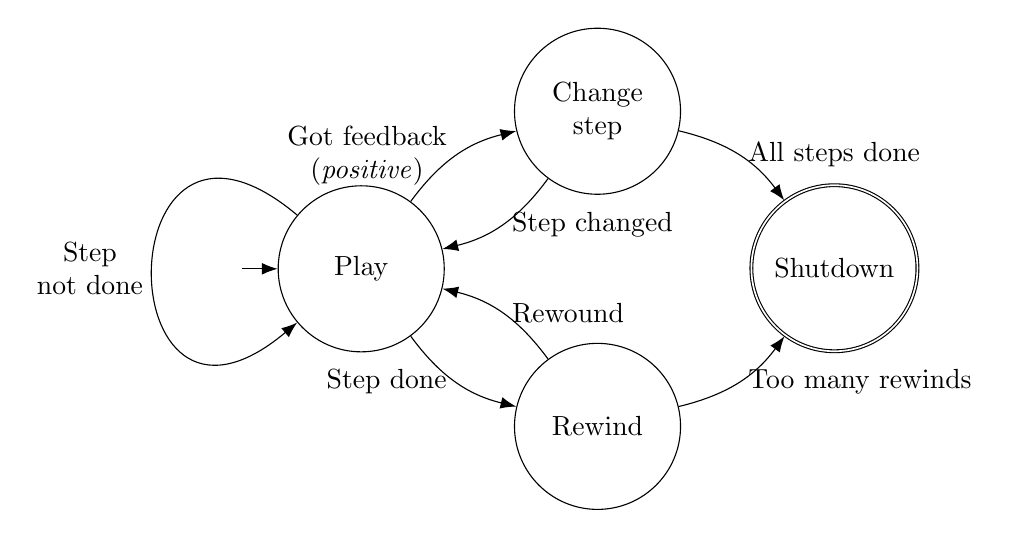
\begin{tikzpicture}[align=center,
        node distance=.5cm and 1.5cm,
        every initial by arrow/.style={-{Latex[length=2mm]}}]
        % Place nodes              
        \node [initial, state, minimum size=6em, initial text=] (play) {Play};               
        \node [state, above right=of play, minimum size=6em] (change) {Change\\step};
        \node [state, below right=of play, minimum size=6em] (rewind) {Rewind};
        \node [state, accepting, above right=of rewind, minimum size=6em] (shutdown) {Shutdown};
        
        
        
        % Draw edges
        \path[draw, -{Latex[length=2mm]}]
        (play) edge [bend right=20] node[left] {Step done} (rewind)
        edge [bend left=20] node[left] {Got feedback\\(\emph{positive})} (change)
        edge [out=140,in=220,looseness=6] node[left] {Step\\not done} (play)
        
        (change) edge [bend left=20] node[right] {Step changed} (play)
        edge [bend left=20] node[right] {All steps done} (shutdown)
        
        (rewind) edge [bend right=20] node[right] {Rewound} (play)
        edge [bend right=20] node[right] {Too many rewinds} (shutdown);
        
        \end{tikzpicture}
    }
    \caption{State diagram of the user model}\label{paper:olguinmunoz2018demo:fig:usermodel}
\end{figure}

%A state diagram for the behavior of this user can be seen in \cref{paper:olguinmunoz2018demo:fig:usermodel}.

% Finally, by enabling this benchmark suite to run on commodity-of-the-shelf hardware, in our example we implemented the suite as an Android app, costs can furthermore be reduced by avoiding expensive gadgets to be available. 
% The suite is also based on a well-established cognitive assistance application framework, \emph{Gabriel} \cite{Chen:EarlyImplementation,Ha:TowardsWearableCogAssist}, which we believe will further aid in its adoption.

% In the following, we discuss the architecture and implementation of our benchmarking suite in more detail in particular with respect to wearable cognitive assistance applications.
% However, we stress that our methodology and in fact also our benchmark suite is applicable to most human-in-the-loop application as long as the backend code is available and the sensory input data can be captured.
% \footnote{We plan to make the benchmarking suite available to the community as Free and Open Source Software. Additionally, we plan to release the recorded traces under a Creative Commons License.}

\subsection{Architecture}

The suite has three elements, as shown in \cref{paper:olguinmunoz2018demo:fig:TraceReplayArch}:
% the \emph{application backend}, the \emph{client emulator}, and the \emph{control backend} or \emph{server}, which interact in the following ways:

\begin{description}[labelindent=\parindent, listparindent=\parindent, style=unboxed, leftmargin=0cm]
  \item [The application backend] consists of instances of the target application running on Docker containers. 
  These correspond to real, unaltered instances of said cognitive assistance applications -- we do not model or emulate them in any way -- and they are containerized in order to be able to execute an arbitrary number of them on the same cloudlet.
  \item [The client emulator] consists of an Android application which emulates the behavior of a user operating the target cognitive assistance application while following the previously discussed user model.
  This Android app replays the previously recorded sensory data over the network to a specific \emph{application backend}, while collecting statistics and measurements of the system status. 
  %{\color{blue} Junjue: Should there be an application client in the picture? Logically, the benchmark android app feeds the application client the sensory information it needs, almost like hijacking the camera stream.}
  \item [The control backend] also runs on the cloudlet, although it could be executed in a separate cloud or cloudlet. It controls the execution of the experiments, by controlling the \emph{client emulators} over the network, initializing the \emph{application backends} and finally aggregating collected data when the experiments are completed. 
\end{description}

\begin{figure}
  \centering
  \includegraphics[width=.7\columnwidth]{publications/2018DemoScalingOnTheEdge/img/TraceReplay_GenArch}
  \captionof{figure}{General architecture of the benchmarking suite.}\label{paper:olguinmunoz2018demo:fig:TraceReplayArch}
\end{figure}

\section{Demo Overview}

We will demonstrate the benchmarking framework using the \emph{LEGO Task Guidance} application previously developed by \textcite{chen2015early}.
This application guides a user step by step in the assembly of a LEGO model; input consists exclusively of video feed of the current state of the assembly, whereas feedback includes visual and auditory components in the form of animations and speech, respectively.

The benchmarking tool will be employed to extract key real-time metrics from this application, \emph{e.g.} average computation and network times, as well as the estimated \emph{user experience} level of the system as a whole (\emph{flawless}, \emph{impaired} or \emph{unusable}, based on the categorization in~\cite{chen2017empirical}).

\section{Discussion and Future Work}

Some open questions and challenges remain to be tackled in the design and development of the presented tool.
To start with, the benchmarking suite is relatively narrow in the types of applications it can be applied to, currently only targeting event based cognitive assistance applications.
The tool needs to be extended to work on a much a broader spectrum of applications, in particular those that do not have a clear task model.
Furthermore, the current implementation does not support hardware accelerators (e.g. \glspl{GPU}) that are commonly used for \gls{DNN} inference.

In addition, our current user model is simplistic. 
This model could be expanded to emulate a human user more accurately and realistically, e.g.\ making mistakes and responding to feedback to correct them.

We plan to extend our work in two directions. First, in addition to emulating user behaviors, we plan to simulate all the components in the system in order to generate reproducible experiments, test individual components of a real system, and identify performance bottlenecks when many users are using an application concurrently. Second, we are going to develop a statistical characterization of the application footprint, based on the data obtained from the tool.

\thesispaper{EdgeDroid}{Olguin:EdgeDroid2019}

\thesispaper{Impact of delayed response on WCA}{Olguin:ImpactWCA2021}

\input{publications/2021ImpactDelayedResponse/body.tex}
\thesispaper{CLEAVE}{olguinmunoz2022cleave}

%Benchmarking human-in-the-loop applications is complex.
%This limits reproducibility as well as feasibility of performance evaluations.
%In this paper we present EdgeDroid, a benchmarking suite that addresses these challenges.
%Our core idea rests on recording traces of these applications \jjw{-> application traces} which are then replayed out \jjw{remove out} in a controlled fashion based on an underlying model of human behavior \jjw{-> emulating human behaviors}.
%The traces are then exposed to the original backend compute process of the respective human-in-the-loop application, generating realistic feedback.
%This allows for an automated system that greatly simplifies benchmarking large scale scenarios.
%Our results confirm the utility of EdgeDroid as a tool for system designers, application developers and researchers.

%\jjw{Alternative version:
Many emerging mobile applications, including \acf{AR} and \acf{WCA}, aim to provide seamless user interaction. 
However, the complexity of benchmarking these human-in-the-loop applications limits reproducibility and makes performance evaluation difficult. In this paper, we present EdgeDroid, a benchmarking suite designed to reproducibly evaluate these applications.

Our core idea rests on recording traces of user interaction, which are then replayed at benchmarking time in a controlled fashion based on an underlying model of human behavior. 
This allows for an automated system that greatly simplifies benchmarking large scale scenarios and stress testing the application.
Our results show the benefits of EdgeDroid as a tool for both system designers and application developers.
%}
\section{Introduction}\label{paper:olguinmunoz2022cleave:intro}

The number and applications of \glspl{CPS}~\cite{rajkumar2010cyber} --- i.e.\ systems in which a real, physical mechanism is controlled by a computer --- have exploded in recent years.
However, this rapid increase in adoption has mostly been limited to industrial contexts.
Although \glspl{CPS} present huge opportunities for all facets of society, they have yet to reach our daily lives in any relevant scale due to their stringent operational requirements.
This is about to change, however, as with the advent of novel wireless communication technologies as well as networking paradigms, such as cellular 5G and edge computing~\cite{satyanarayanan2017emergence}, consumer-grade \glspl{CPS} will be made possible.
These technologies meet two key requirements of \glspl{CPS}: real-time capabilities (through extremely low end-to-end latencies), and context- and locality-awareness, and will most likely become the backbone of \gls{CPS} in the future.

\glspl{NCS}~\cite{gupta2010networked}, a type of \gls{CPS} wherein multiple networked actuators and sensors form a part of the same automatic control system will benefit from the adoption of these technologies.
Depending on the physical system being controlled, \glspl{NCS} can have stringent timing and reliability requirements for communication that conventional cloud paradigms and cellular networks cannot meet~\cite{wan2020efficient}.
This necessitates sophisticated tools for the performance evaluation of future system architectures, as well as novel NCS design paradigm.

%Due to their potential advantages for industrial and commercial settings, there exist works~\cite{Zhang2016Survey} dedicated to the modelling and performance characterization of \glspl{NCS}, improving NCSs by distributing control functions across networks, facilitating centralized coordination, control, and monitoring.

One the one hand, related literature in \glspl{NCS} leverages to a large extent theoretical models, at the price of being able to capture networked systems effects only on a coarse level.
%follows a theoretical approach, and only a small fraction of it deals with experimental studies.
On the other, there exist several approaches when considering experimental methodologies. 
%A number of works concerning \glspl{NCS} deal with experimental studies.
%\glspl{NCS} have an inherently inter-domain nature intertwining knowledge from the fields of communications, computing, and control theory in ways that cannot be studied in isolation, leading to various different approaches to such studies.
One such approach uses setups in which the complete system is built on top of real hardware.
This approach is employed in the works of Baumann \emph{et al.}~\cite{baumann2018evaluating} and Cuenca \emph{et al.}~\cite{cuenca2019periodic}; in both of these, the authors implement their approach on physical testbeds.
Conversely, other studies choose to instead use completely \emph{simulated} \gls{NCS} setups.
The authors in\ \cite{ma2019optimal} have opted for such an approach.
These studies often employ combinations of physical and network simulation tools trying to capture the complex dynamics of \glspl{NCS}.
Finally, some experimental studies instead employ \emph{virtualized} approaches, in which either
\begin{enumerate*}[itemjoin={{; }}, itemjoin*={{; or }}]
    \item a real network interacts with a simulated or emulated control system~\cite{wang2020inverter}
    \item a simulated network interacts with a real control system~\cite{natale2004inverted}.
\end{enumerate*}

As evidenced above, experimental research in \glspl{NCS} includes varied heterogeneous hardware and software platforms, methodologies and key performance indicators.
This, in turn, leads to hardware, software, and methodology fragmentation, as different studies tend to prefer approaches more favored in their respective communities.
Furthermore, existing studies tend to focus on individual aspects and components of a system, thus producing results which do not provide a complete image of the \gls{NCS}.
This has caused a gap in knowledge pertaining to the reproducibility and comparison of experimental studies on these systems.

Zoppi \emph{et al.}~\cite{zoppi2020ncsbench} made the first (and to the best of our knowledge, the only) attempt at tackling this challenge in their work.
In their work, they proposed a platform called NCSBench, to be used for reproducible benchmarking in NCS.\ 
Their methodology utilizes joint knowledge of control, computation, and communication. 
In their work various architectural elements and the corresponding delays associated with the NCS are modelled. 
Multiple experimental parameters and certain observable key performance indicators are defined and utilized in the implementation. 
This work however utilizes a physical LEGO\textregistered{}\ Mindstorms EV3 Core Set\texttrademark{}\  based plant for the implementation, preventing instantaneous changes in plant characteristics and component parametrizations.
Furthermore, relying on physical objects like an inverted pendulum limits scalability of the experimentation in practice. 

We overcome this issue by proposing a completely virtual plant allowing for unparalleled flexibility in changing the plant model and characteristic features of the experiments.
In this paper, we present the first fully-software-based framework for scalable and repeatable benchmarking of edge-native \gls{NCS}.
As edge computing begins being adopted by industry, more and more variations have begun to appear in literature.
``Near'', ``far'', ``core'', and ``telco'' edge describe variations of the original concept and are becoming ubiquitous in new research.
While the core idea of edge computing is widely accepted as fundamental for pervasive \glspl{NCS} in general, understanding the strengths and weaknesses of such different edge concepts is of paramount importance.

Our framework, \gls{CLEAVE}, aims to simplify the repeatable and scalable benchmarking of such systems.
It is fully virtualized, inspired by our previous work on benchmarking human-in-the-loop applications on the edge~\cite{olguinmunoz2019edgedroid}.
The tool consists of a benchmarking framework and software development kit for the development of emulated physical systems and softwarized controllers.
These virtual \glspl{NCS} can then be deployed on real networks for reparametrizable, repeatable, and reproducible benchmarking of the complete system.

\gls{CLEAVE} is built using \emph{Python 3.8}, making it highly extensible and able to harness the multitude of already existing user libraries.
It is furthermore compatible with container technologies such as \emph{Docker}\footnote{Docker Engine: \url{https://www.docker.com/}}, making it suitable for automated deployment, scaling, and benchmarking on industry-standard edge setups using container orchestration solutions.

The rest of this paper is structured as follows.
\cref{paper:olguinmunoz2022cleave:approach} presents the design principles and implementation of the framework.
In \cref{paper:olguinmunoz2022cleave:experiments}, we present a use case scenario which validates the utility, flexibility, and repeatability of \gls{CLEAVE}.
Finally, in \cref{paper:olguinmunoz2022cleave:conclusion} we conclude this work.

\input{publications/2022CLEAVE/cleave.tex}
\section{Use case validation}\label{paper:olguinmunoz2022cleave:experiments}

In this section, we demonstrate the utility of \gls{CLEAVE} by walking readers through an example use case.
With this, we aim to showcase the ability of our framework to provide accurate and repeatable measurements of the performance of \glspl{NCS} deployed on edge computing infrastructure.

We present the following use case scenario.
A simple \gls{NCS} consisting of an \emph{inverted pendulum} plant controlled by a \emph{proportional-differential} controller is to be deployed on an Edge server.
The connection between plant and server is over a WiFi (IEEE 802.11n) link.
Moreover, there are a number of video-streaming applications running concurrently on the Edge setup.

We believe this to be an interesting and representative use-case scenario for a number of reasons.
Firstly, the inverted pendulum is broadly used as a benchmark in control-system literature, see for instance\ \cite{baumann2018evaluating} and\ \cite{natale2004inverted}.
A key reason for this is that such a relatively simplistic system allows for straightforward reparametrization to obtain varied system dynamics, which in turn makes a broader range of experiments possible.
Secondly, similar, albeit non-Edge-enabled, setups have been a reality in industry for almost two decades, as evidenced by\ \cite{gupta2010networked}.
Thirdly, although real deployments would most assuredly employ mobile technologies due to the added benefits of mobility and range, the \glspl{RTT} offered by these technologies are higher, or at best equal, those offered by WiFi.
4G, for instance, has average \glspl{RTT} of around a few hundred milliseconds, which is orders of magnitude greater than the values measured in our scenario, and current 5G deployments offer \gls{RTT} values barely matching the sub-\SI{10}{\milli\second} values we obtain for WiFi.
Thus, we argue that using WiFi allows for more experimental freedom, as the system can be tweaked to obtain worse \glspl{RTT} more akin to those of mobile technologies while still having the option to study best-case scenarios with very low-latencies.
Finally, video analytics is one of the main proposed use cases for edge computing~\cite{ananthanarayanan2017real,yi2017lavea,wang2018bandwidth}, and thus we foresee edge \gls{NCS} deployments being deployed in parallel with such applications in the future.
However, before deployment can become a reality, key questions such as: 
``what are the baseline requirements of the \gls{NCS}?'';
``what are the achievable best-case end-to-end latencies in the system?'';
and ``how does the concurrent video-streaming traffic affect \gls{NCS} stability?'' need to be answered.

We attempt to study these questions using the experimental setup in \cref{paper:olguinmunoz2022cleave:fig:cleave:expsetup}.
\gls{CLEAVE} is deployed on a testbed consisting of \num{10} Raspberry Pi 4B  clients connected wirelessly to an IEEE 802.11n \gls{AP}.
Connected to the Ethernet backbone of this \gls{AP} is a general-purpose \verb|x86_64| desktop computer acting as a Cloudlet/Edge server.

% \input{tables/hardware.tex}

\begin{figure}
    \centering
    \includegraphics[width=.95\textwidth]{publications/2022CLEAVE/images/CLEAVE_experiment_setup}
    \caption{
        The setup used for our experimentation. 
        % Containerized versions of the core CLEAVE emulation components are deployed inside a Docker Swarm Overlay Network spanning \num{10} Raspberry Pi 4B clients connected to a single Cloudlet over an IEEE 802.11n \gls{AP}.
    }\label{paper:olguinmunoz2022cleave:fig:cleave:expsetup}
\end{figure}

The first step in our case study is to evaluate the baseline performance of the control system, both locally and over the network.
We configure \gls{CLEAVE} to run a single loop with both plant and controller co-located on the Edge server, and we also configure a separate setup with an identical loop executed over the wireless link.
For both of these setups, we execute a series of scenarios varying:
\begin{enumerate*}[itemjoin={{; }}, itemjoin*={{; and }}]
    \item the sampling rate of the Plant state, setting it to \SIlist[list-final-separator={, or }]{5;10;20;40;60}{\hertz}
    \item the responsiveness of the Controller, adding fixed delays of \SIlist[list-final-separator={, or }]{0;25;50}{\milli\second} after the processing of each sample.
\end{enumerate*}

We run repeated executions of each combination of these parameters at least \num{10} times, for both the networked and ``local-only'' setups.
Each execution lasts for \SI{5}{\minute}, during which we collect detailed data on both the state of the controlled system as well as on the data sent over the network.
After the initial \num{10} runs, we identify that setups with sampling rates of \SIlist{5;10}{\hertz} were consistently too unstable to consider, and disregard them in further analyses.
We further note that setups with \SI{0}{\milli\second} additional delay are always stable and thus also disregard them.
Remaining setups, i.e.\ sampling rates \( \geq \) \SI{20}{\hertz} and artificial delays \( \geq \) \SI{25}{\milli\second}, are repeated an additional \num{20} times for better statistical significance.

This repeated experimentation and data collection while ``zooming in'' on particular setups is facilitated by \gls{CLEAVE}s design.
Scenarios are executed automatically in batches using a simple Python script which interacts with Docker through the widely adopted \emph{docker-py}\footnote{Docker SDK for Python: \url{https://docker-py.readthedocs.io/en/stable/}} library.
This is \gls{CLEAVE}s first advantage over existing frameworks;
it is designed with cloud and edge technology and paradigms in mind, making integration with existing systems convenient.

\begin{figure}[t]
    \centering
    \begin{subfigure}[t]{.7\textwidth}
        \centering
        \includegraphics[width=\textwidth]{publications/2022CLEAVE/plots/fixed_single_loop_toppled}
        \caption{Fraction of toppled plants.}\label{paper:olguinmunoz2022cleave:fig:single:topple}
    \end{subfigure}\\
    \begin{subfigure}[t]{.7\textwidth}
        \centering
        \includegraphics[width=\textwidth]{publications/2022CLEAVE/plots/fixed_single_loop_rms}
        \caption{Mean angle \gls{RMS}; red line indicates \( y = 180 \).}\label{paper:olguinmunoz2022cleave:fig:single:rms}
    \end{subfigure}\\
    \begin{subfigure}[t]{.7\textwidth}
        \centering
        \includegraphics[width=\textwidth]{publications/2022CLEAVE/plots/fixed_single_loop_rtts}
        \caption{
            Mean \glspl{RTT}.
        }\label{fig:single:rtt}
    \end{subfigure}%
    \caption[caption]{
        Baseline results.
        Error bars indicate \SI{95}{\percent} \glspl{CI}.
        }%
    \label{paper:olguinmunoz2022cleave:fig:single}
\end{figure}

\cref{paper:olguinmunoz2022cleave:fig:single} shows a summary of the results relating to the single-loop scenarios:
\cref{paper:olguinmunoz2022cleave:fig:single:topple} shows the fraction of plants that toppled in each scenario, and \cref{paper:olguinmunoz2022cleave:fig:single:rms} shows the average \gls{RMS} for the absolute pendula angles.
\cref{fig:single:rtt} shows average latency due to network and processing (excluding synthetic delays) for both single-loop scenarios.
Packet losses were below \SI{0.2}{\percent} for all parametrizations of the single-loop scenario over the network, and \SI{0}{\percent} for all parametrizations of the local-only setup.

As expected, higher sampling rates tend to correlate with better quality of control;
at higher sampling rates the system was able to reach stability at higher \glspl{RTT}.
These initial results already hint at interesting consequences for such an edge-bound \gls{NCS} deployment.
For instance, it is clear from \cref{paper:olguinmunoz2022cleave:fig:single:topple,paper:olguinmunoz2022cleave:fig:single:rms} that network delays can, to a certain extent, be compensated for by increasing the sampling rate of the system.
A corollary of this is, conversely, that at lower network latencies \glspl{NCS} are able to stabilize at lower sampling rates.
Adaptive sampling might thus be a viable method for optimizing resource utilization.

Once baselines for single loops in the use case scenario have been established, we can proceed to studying the interaction between the \glspl{NCS} and the video-streaming applications.
We deploy \num{6} control loops on the experimental setup depicted in \cref{paper:olguinmunoz2022cleave:fig:cleave:expsetup}.
On the remaining \num{4} clients we run the \emph{iperf3}\footnote{iperf3: \url{https://iperf.fr/}} traffic load generator, each generating \SI[per-mode=symbol]{6.5}{\mega\bit\per\second} of uplink \gls{UDP} traffic.
This emulates the load generated on the network by \SI{1080}{p} Full-HD video streaming, originating from the clients and terminating in the cloudlet.
Based on the baseline results, we execute setups with \gls{NCS} plant sampling rates of \SIlist{20;40;60}{\hertz}.
Each sampling rate configuration is run for \SI{5}{\minute}, and then repeated \num{30} times to obtain statistical significance.
Once again, repetitions of this scenario are executed automatically in batches using a simple Python script and \emph{docker-py}.

\begin{figure}[t]
    \centering
    \begin{subfigure}[h]{.5\textwidth}
        \centering
        \includegraphics[width=.8\textwidth]{publications/2022CLEAVE/plots/fixed_video_topple_frac}
        \caption{Toppled plants.}\label{paper:olguinmunoz2022cleave:fig:video:toppled}
    \end{subfigure}%
%    \hfill%
    \begin{subfigure}[h]{.5\textwidth}
        \centering
        \includegraphics[width=.8\textwidth]{publications/2022CLEAVE/plots/fixed_video_angle_rms}
        \caption{Angle \gls{RMS}.}\label{paper:olguinmunoz2022cleave:fig:video:rms}
    \end{subfigure}\\
    \begin{subfigure}[h]{.5\textwidth}
        \centering
        \includegraphics[width=.8\textwidth]{publications/2022CLEAVE/plots/fixed_video_drop_frac}
        \caption{Packet losses.}\label{paper:olguinmunoz2022cleave:fig:video:drop}
    \end{subfigure}%
%    \hfill%
    \begin{subfigure}[h]{.5\textwidth}
        \centering
        \includegraphics[width=.8\textwidth]{publications/2022CLEAVE/plots/fixed_video_rtt}
        \caption{\glspl{RTT}.}\label{paper:olguinmunoz2022cleave:fig:video:rtt}
    \end{subfigure}%
    \caption{
        Multi-loop, resource-constrained setup results.
        Error bars indicate \SI{95}{\percent} \glspl{CI} in all plots.
    }\label{paper:olguinmunoz2022cleave:fig:video:results}
\end{figure}

\cref{paper:olguinmunoz2022cleave:fig:video:results} shows a summary of the results obtained.
\cref{paper:olguinmunoz2022cleave:fig:video:toppled} shows the fraction of repetitions of each setup in which \emph{at least} one plant failed to maintain stability and toppled.
\cref{paper:olguinmunoz2022cleave:fig:video:rms} shows the \gls{RMS} for the pendulum angles for each setup, only considering data from plants that did not topple.
\cref{paper:olguinmunoz2022cleave:fig:video:drop} shows the fraction of \gls{UDP} datagrams dropped, averaged over all plants and repetitions per setup.
\cref{paper:olguinmunoz2022cleave:fig:video:rtt} shows the measured end-to-end plant-side \gls{RTT}, averaged over all plants and repetitions per setup.

These results are interesting in their counter-intuitiveness compared to the single-loop baseline results.
While the baselines might lead us to think that higher sampling rates are always better for the stability of control systems, \cref{paper:olguinmunoz2022cleave:fig:video:toppled,paper:olguinmunoz2022cleave:fig:video:rms} show this not to be the case for \gls{NCS} in resource-constrained scenarios.
\SI{60}{\hertz} was the least stable configuration, with at least one pendulum toppling in around \SI{16}{\percent} of the repetitions, and mean pendulum angle \gls{RMS} circa \num{3} times that of the \SI{40}{\hertz} scenario.
\SI{40}{\hertz} was in turn the second worst configuration --- although it presented no toppled pendula, average angle \gls{RMS} doubled that of the \SI{20}{\hertz} setup.

\cref{paper:olguinmunoz2022cleave:fig:video:drop,paper:olguinmunoz2022cleave:fig:video:rtt} explain these behaviors.
Whereas both the \SIlist{20;40}{\hertz} setups show losses well below \SI{5}{\percent}, the \SI{60}{\hertz} scenario shows an average of around \SI{13}{\percent} of datagrams lost.
The differences in \glspl{RTT} results are equally telling; \glspl{RTT} for the \SI{60}{\hertz} setup were on average approx.\ \num{3} times those for the \SIlist{20;40}{\hertz} setups.
These results stem from the contention for network resources, and hint at important trade-offs system designers will have to take into consideration when designing and developing \glspl{NCS} for deployment on the Edge.
The Edge will be \emph{multi-tenant} and \emph{multi-instance}. 
\gls{NCS} deployments will have to be designed with shared resources in mind, and given the complexity of these systems, experimental tools like \gls{CLEAVE} will be key for their succesful adoption and massification.

\section{Conclusions and Future Directions}\label{paper:olguinmunoz2022airnur:conclusion}

In this paper, we have introduced a framework for repeatable end-to-end testbed automation in the context of wireless networking and edge computing research.
Named Ainur, it simplifies the execution and verification of end-to-end experimentation by automating the
\begin{enumerate*}[itemjoin={{; }}, itemjoin*={{; and }}]
    \item establishment of physical links between hosts, including the configuration of complex wireless systems such as 4G \gls{LTE} and 5G
    \item provisioning of and connection to remote cloud instances
    \item initialization of \gls{IP} layer connectivity between hosts
    \item collection of logs and data
    \item deployment, scaling, and lifecycle management of containerized processes
\end{enumerate*}.
We have described its general architecture, which follows a layered design mimicking the network stack layers the framework directly interacts with, as well as the underlying assumptions about its deployment environment and specific requirements for its deployment.
We have also outlined a demonstration which showcases the flexibility and power of the framework by deploying two different workloads to our testbed.
We believe our framework represents an important step towards repeatable, replicable, yet low-access barrier end-to-end wireless testbed experimentation.
It has been released as \gls{FOSS} and can be found on GitHub~\cite{ainur:github}.\\

In terms of future work, our current efforts are focused on the expansion and integration of Ainur with \gls{CHI}~\cite{keahey2020lessons}.
While we believe Ainur to be unique and valuable in its focus on fully-automated end-to-end wireless edge computing experimentation, integrating with the above software stacks will provide a number of features and functionalities which will greatly expand Ainur's potential.
Features like resource reservation, multi-tenant testbed access, and automated bare-metal and \gls{VM}-host instantiation will make Ainur better suited for larger scale experimentation and allow us to expand the research domain targeted by the framework.
Our ultimate goal is to eventually provide Ainur as a service running inside an OpenStack/\gls{CHI} environment, leveraging the flexibility of the platform to automate the reservation of resources, instantiation of nodes and networks, execution of experiments, and final collection of results.

\section*{Acknowledgements}\label{paper:olguinmunoz2022cleave:acks}

This research has been partially funded by
\begin{inlineenum}
    \item the VINNOVA Competence Center for \gls{TECoSA} at KTH Royal Institute of Technology
    \item the \gls{SSF}, through grant number \verb|ITM17--0246|.
\end{inlineenum}

We also wish to thank S.~S.~Mostafavi, V.~N.~Moothedath, M.~Alsakati, O.~Ferm, S.~Vojcic, and A.~Bhattacharya for their support and valuable contributions to this work.

Finally, we would like to thank the reviewers for their insightful comments and suggestions, which greatly helped us improve this work.


\section*{References}
\addcontentsline{toc}{section}{References}
\newrefcontext[sorting=ynt]{}
\printbibliography[
    heading=none,
    category=thesispapers
]{}
\newrefcontext[sorting=appearance-date-name]{}
\printbibliography[
    heading=none,
    notcategory=thesispapers
]{}
\end{appendices}

\end{document}
\endinput
%%
%% End of file `kth-demo.tex'.
